\documentclass{article}
\usepackage{rlj}

\usepackage{booktabs}
\usepackage{graphicx}
\usepackage{amssymb,amsfonts}
\usepackage{amsthm}
\usepackage{subcaption}
\usepackage{xcolor}
\usepackage{colortbl}
\usepackage{pgfplots}
\pgfplotsset{compat=1.18}
\usepackage{tikz}
\usepackage{appendix}

\title{Do Recurrent RL Agents Discover a Unique Internal Clock?\\Evidence Against a Canonical Temporal Code}

\author{Anonymous Authors}

\setrunningtitle{Do Recurrent RL Agents Discover a Unique Internal Clock?}

\keywords{temporal representation, recurrent neural networks, reinforcement learning, representational analysis, CKA}

\summary{
We examine how LSTM-based RL agents frame temporal information in their hidden states when no explicit clock is provided.
Using CKA comparison with engineered encodings, linear probing, and PCA, we find that temporal encoding is training-dependent, non-unique across random seeds, and sensitive to temporal horizon.
These findings challenge the implicit assumption that recurrent networks discover a single canonical temporal code, and suggest that the framing of time in learned representations is contingent on optimization path and task structure.
}

\contribution{We show that temporal encoding in recurrent RL agents is not unique—different training runs produce different internal clocks despite identical behavior.}{Challenges the implicit ``canonical temporal code'' assumption in RL representation analysis.}
\contribution{We demonstrate that the representational geometry shifts with temporal horizon, from sinusoidal-like to scalar-like encoding.}{Links task structure to the learned framing of time, with implications for transfer and generalization.}
\contribution{We provide a simple, controlled methodology (CKA against engineered codes + multi-seed comparison) for testing uniqueness assumptions about learned representations.}{Applicable beyond time to other latent task variables.}

\begin{document}

\makeCover
\maketitle

\begin{abstract}
Recurrent RL agents that must track time without an explicit clock have to invent their own internal framing of the temporal dimension.
A natural assumption is that this framing is unique---that any sufficiently trained agent converges to the same canonical temporal code.
We show this assumption is wrong: LSTM agents trained on the same periodic task construct fundamentally different internal representations of time depending on their random initialization.
Using Centered Kernel Alignment (CKA) against engineered temporal encodings, linear probing, and PCA on DoorGrid, an environment with periodic dynamics, we ask three questions: (Q1) Is temporal structure learned or inherent to recurrence?
(Q2) Is the emergent encoding unique across training runs?
(Q3) How does the encoding depend on the temporal horizon?
A random-weight LSTM control shows that temporal structure is weak before training (CKA $\approx 0$, phase accuracy at chance) but emerges reliably after RL training.
Multi-seed experiments ($T = 4$, 5 seeds) reveal that the learned encoding is \emph{non-unique}: all agents achieve perfect timestep prediction (R$^2 = 1.0$) yet exhibit different CKA profiles---the highest-CKA engineered encoding varies across seeds from sinusoidal positional encoding to phase-based encoding.
A controlled horizon manipulation ($T \in \{4, 8, 16, 32\}$, 5 seeds each) shows that representation similarity is \emph{horizon-sensitive}: CKA with raw scalar encoding increases from $0.40 \pm 0.10$ at $T = 4$ to $0.70 \pm 0.22$ at $T = 32$, while sinusoidal PE decreases from $0.63 \pm 0.09$ to $0.50 \pm 0.08$.
These findings challenge the implicit assumption that recurrent networks converge to a single canonical temporal code; the framing of time in learned representations is contingent on both initialization and task structure.
\end{abstract}

\section{Introduction}

RL researchers typically assume the hidden state of a recurrent network is a unified representation of the agent's situation---including elapsed time.
But when no clock signal is provided, the agent has to \emph{construct its own framing} of the temporal dimension.
This invites a question: given a well-defined POMDP, do trained agents converge to a \emph{canonical} temporal code---a unique, reproducible internal clock?
Our answer is no: different training runs produce different temporal codes despite identical behavioral performance.

Prior work has established that time cells emerge in RNN-based RL agents, analogous to hippocampal time cells \citep{macdonald2011hippocampal,lin2023timecells}.
In NLP, the form of positional encoding---sinusoidal, learned, or relative---has been a central design choice in the Transformer architecture \citep{vaswani2017attention}.
Less is known about the \emph{variability and contingency} of such representations in recurrent RL agents.

We address three concrete questions:
\begin{enumerate}
\setlength{\itemsep}{0pt}
\item[(Q1)] Does temporal structure emerge through training, or is it inherent to recurrent architectures?
\item[(Q2)] Is the emergent encoding unique across training runs?
\item[(Q3)] How does the encoding depend on the temporal horizon of the task?
\end{enumerate}

We study these questions by training LSTM agents on DoorGrid, an environment with periodic dynamics, and comparing their hidden states against a library of engineered temporal encodings using Centered Kernel Alignment (CKA) \citep{kornblith2019cka}, complemented by linear probing, PCA, and single-neuron phase selectivity analysis.

Our central finding is that the temporal framing learned by LSTM agents is \emph{non-unique}: agents with identical task performance align differently with simple engineered temporal codes, and the preferred alignment shifts with temporal horizon.
This calls into question how we interpret and compare recurrent representations across training runs---if there is no single canonical code, what exactly are we comparing?

\section{Related Work}

\subsection{Temporal Representations in RL}

\citet{lin2023timecells} showed that time cells emerge in RNN-based RL agents, extending the neuroscience observation that hippocampal neurons encode elapsed time \citep{macdonald2011hippocampal}.
\citet{hausknecht2015drqn} introduced DRQN, showing that recurrent connections enable RL agents to handle partial observability.
\citet{kapturowski2019r2d2} scaled this with R2D2 using LSTM-based agents on Atari.
\citet{jaderberg2017aux} showed that auxiliary temporal prediction tasks improve representation learning.
Our work examines not just \emph{whether} agents encode time, but whether this encoding has a unique canonical form.

\subsection{Probing Neural Representations}

Linear probing \citep{alain2017probe} and CKA \citep{kornblith2019cka} are standard tools for analyzing representations.
\citet{hewitt2019designing} emphasized that probe accuracy alone is insufficient---one must control for selectivity.
\citet{voita2020information} studied information-theoretic aspects of probing.
CKA is used here as a descriptive similarity measure to a small library of candidate temporal codes, not as an identification procedure for the true latent code.

\subsection{Multiple Solutions in Neural Networks}

The existence of multiple loss landscape basins is well documented \citep{garipov2018loss,li2018visualizing,draxler2018essentially}.
In neuroscience, \citet{edelman2001degeneracy} formalized \emph{degeneracy}---distinct structures performing the same function.
We ask a question that sits at the intersection of these lines of work: do different optimization basins produce qualitatively different \emph{temporal representations} for the same RL task?

\section{Methods}

\subsection{Environment}

\textbf{DoorGrid} is an 8$\times$8 grid with a periodic door that alternates between open and closed.
At $T = 4$, the door is open during phases 0--1 and closed during phases 2--3.
The agent receives a one-hot encoding of its $(x, y)$ position (64-dimensional); no explicit temporal features are provided.
Actions are $\{$up, down, left, right$\}$.
The reward is $+1$ for reaching the goal (top-right corner), $-1$ for stepping into a hazard (a cell that is terminal when the door is closed), and $0$ otherwise.
Episodes terminate upon reaching the goal, hitting a hazard, or exceeding a step limit.
For horizon scaling, we vary $T \in \{4, 8, 16, 32\}$; the door is open during the first half of each period and closed during the second half.

We chose this minimal environment deliberately: the periodic temporal structure is the agent's primary challenge, letting us isolate temporal encoding from complex spatial navigation.

\subsection{Agents and Training}

A single-layer LSTM ($d = 64$) with linear policy and value heads, trained with REINFORCE with baseline (learning rate $10^{-3}$, entropy coefficient 0.01, discount $\gamma = 0.99$).
An MLP baseline (2-layer, 64 units each) processes each observation independently, serving as a sanity check for the necessity of recurrence.
All experiments use 5 random seeds $\{42, 123, 456, 789, 1024\}$.

\subsection{Analysis Pipeline}

After training, we run 200 evaluation episodes and collect hidden state vectors $\mathbf{h}_t \in \mathbb{R}^{64}$ along with timestep $t$ and phase $\phi = t \bmod T$.

\textbf{Linear Probe.}
Ridge regression from $\mathbf{h}_t$ to $t$ (R$^2$ score) and logistic regression to $\phi$ (classification accuracy), with shuffled-target controls ($R^2_{\text{shuffled}} = 0.020$, confirming no leakage).

\textbf{PCA.}
PC1 variance fraction and its correlation with timestep.

\textbf{Mutual Information.}
Normalized mutual information $I(h_d; \phi) / H(\phi)$ between each hidden dimension and phase, averaged over dimensions, quantifying how much phase information is distributed across the representation.

\textbf{CKA.}
Linear CKA \citep{kornblith2019cka} between $\mathbf{h}_t$ and engineered temporal encodings: raw scalar ($t/T$), sinusoidal PE ($\sin/\cos$ of $2\pi t/T$), phase sin/cos, one-hot phase, and remaining time ($(T-t)/T$).
As reference baselines, CKA between engineered encodings themselves ranges from $0.38$ to $0.54$ at $T = 8$, and CKA between any encoding and shuffled hidden states is approximately $0$.

\textbf{Single-Neuron Phase Selectivity.}
For each hidden dimension $d$, we compute the mean activation per phase $\bar{h}_d(\phi)$ and a selectivity index $s_d = (\max_\phi \bar{h}_d - \min_\phi \bar{h}_d) / (\max_\phi \bar{h}_d + |\min_\phi \bar{h}_d| + \epsilon)$.
Neurons with $s_d \approx 1$ are strongly phase-tuned.
We compare the top-$k$ phase-selective dimensions across seeds.

\section{Results}

\subsection{Temporal Structure Emerges Through Training (Q1)}
\label{sec:learned}

\begin{table}[t]
\centering
\caption{Trained vs.\ untrained LSTM on DoorGrid ($T = 4$).
R$^2(t)$: timestep prediction. Acc($\phi$): phase classification.
CKA Best: highest CKA with any engineered encoding.
Return: best evaluation reward (20-episode mean).
Trained row shows seed 42 as representative; all 5 seeds achieve R$^2 = 1.0$ and Return $= 0.920$.
Untrained LSTM does not participate in the RL task, so Return is not applicable.}
\label{tab:main}
\begin{tabular}{lccccc}
\toprule
\textbf{Condition} & \textbf{R$^2(t)$} & \textbf{Acc($\phi$)} & \textbf{CKA Best} & \textbf{MI norm} & \textbf{Return} \\
\midrule
Trained (seed 42) & 1.000 & 1.000 & 0.740 & 1.000 & 0.920 \\
Untrained         & 0.304 & 0.298 & 0.153 & 0.082 & N/A \\
\bottomrule
\end{tabular}
\end{table}

Table~\ref{tab:main} speaks to Q1.
Trained LSTMs show strong temporal encoding (R$^2 = 1.0$, CKA $= 0.74$, phase accuracy 1.0) while untrained LSTMs show CKA $\approx 0$ and phase accuracy at chance ($0.30$ for 4 classes).
The temporal structure we measure is largely training-dependent rather than a mere artifact of random recurrent dynamics.
As expected, the MLP baseline (which lacks recurrence) fails to learn the task (Return $= -2.0$, R$^2 < 0.04$), confirming that temporal tracking requires recurrent state.

\subsection{The Temporal Framing Is Not Unique (Q2)}
\label{sec:degenerate}

\begin{table}[t]
\centering
\caption{CKA (mean $\pm$ std across 5 seeds) between DoorGrid ($T = 4$) hidden states and engineered encodings. High std relative to mean indicates seed-dependent encoding. Highest-CKA mean in \textbf{bold}.}
\label{tab:cka}
\begin{tabular}{lc}
\toprule
\textbf{Encoding} & \textbf{CKA (mean $\pm$ std)} \\
\midrule
Raw scalar ($t/T$) & $0.40 \pm 0.10$ \\
Sinusoidal PE      & $\mathbf{0.63 \pm 0.09}$ \\
Phase sin/cos      & $0.28 \pm 0.21$ \\
One-hot phase      & $0.27 \pm 0.16$ \\
\bottomrule
\end{tabular}
\end{table}

All 5 seeds achieve R$^2 = 1.0$, phase accuracy $= 1.0$, and Return $= 0.920$---functionally identical performance.
Yet the CKA profiles differ substantially across seeds.
Of 5 seeds, 4 show highest CKA with sinusoidal PE ($0.64$--$0.74$), while seed 456 shows highest CKA with phase sin/cos ($0.62$) with sinusoidal PE scoring lower ($0.46$).
The coefficient of variation across seeds is $0.15$ for CKA(sin\_PE) and $0.76$ for CKA(phase), indicating that the encoding geometry is sensitive to random initialization.
Cross-seed CKA between the agents' own hidden states (aligned by timestep) is uniformly high ($> 0.96$), so the overall representational geometry is similar across seeds.
The plurality we identify is not in the raw hidden-state structure but in the \emph{alignment with specific engineered codes}: the same population geometry can be more or less similar to different candidate temporal codes depending on initialization.

\textbf{Single-neuron evidence.}
We identify the 8 hidden dimensions with highest phase selectivity ($s_d \approx 1.0$ for all seeds) as ``time cells.''
Across all 10 pairs of seeds, the mean overlap in top-8 time cell dimensions is 1.8/8 (mean Jaccard index $= 0.14$).
However, with 34 of 64 dimensions showing near-maximal selectivity ($s_d > 0.9$), the hypergeometric expectation for random overlap is $8 \times 8 / 34 \approx 1.88$---making the observed overlap indistinguishable from chance.
We therefore do not treat single-neuron overlap as evidence for or against representational plurality; the population-level CKA differences (above) provide the stronger signal.
Because hidden-unit indices are not aligned across independently trained models, we treat the overlap analysis as descriptive (see Appendix~\ref{app:neurons} for per-seed details).

\subsection{The Framing Shifts with Temporal Horizon (Q3)}
\label{sec:horizon}

\begin{table}[t]
\centering
\caption{Representation similarity shifts with temporal horizon in DoorGrid.
CKA (mean $\pm$ std, 5 seeds) with engineered temporal encodings.
$^\dagger$1 seed failed at $T = 16$ and 2 at $T = 32$; stats computed on all 5.
Converged-only: $T\!=\!16$: CKA(raw)$\!=\!0.59$, sin\_PE$\!=\!0.65$; $T\!=\!32$: CKA(raw)$\!=\!0.61$, sin\_PE$\!=\!0.54$.}
\label{tab:scaling}
\begin{tabular}{cccccc}
\toprule
$T$ & \textbf{CKA(raw)} & \textbf{CKA(sin\_PE)} & \textbf{$|$PC1-t$|$} & \textbf{R$^2(t)$} & \textbf{Return} \\
\midrule
4  & $0.40 \pm 0.10$ & $\mathbf{0.63 \pm 0.09}$ & $0.44 \pm 0.10$ & $1.000$ & $0.920$ \\
8  & $0.56 \pm 0.14$ & $\mathbf{0.58 \pm 0.08}$ & $0.46 \pm 0.29$ & $1.000$ & $0.880$ \\
16 & $\mathbf{0.64 \pm 0.15}$ & $0.60 \pm 0.10$ & $0.63 \pm 0.37$ & $1.000$ & $0.800^\dagger$ \\
32 & $\mathbf{0.70 \pm 0.22}$ & $0.50 \pm 0.08$ & $0.71 \pm 0.28$ & $1.000$ & $0.640^\dagger$ \\
\bottomrule
\end{tabular}
\end{table}

Table~\ref{tab:scaling} and Figure~\ref{fig:scaling} answer Q3.
At $T = 4$, mean similarity to sinusoidal PE is highest (CKA $= 0.63$ vs.\ raw scalar $= 0.40$).
At $T = 8$, the two are roughly equal (CKA $\approx 0.57$).
At $T \geq 16$, similarity to raw scalar exceeds sinusoidal PE.
The |PC1-timestep correlation| also increases with period length (from $0.44$ at $T = 4$ to $0.71$ at $T = 32$), indicating that temporal information becomes more concentrated in a single dominant dimension at longer horizons.

The seed-level variability persists across all period lengths.
At $T = 8$, seed 42 shows highest CKA with raw scalar ($0.81$) while seeds 123/456/789 show highest CKA with sinusoidal PE ($0.48$--$0.58$).
At $T = 16$, seed 1024 matches raw scalar ($0.84$) while seed 789 matches remaining time ($0.77$).
The framing of time is not an artifact of a single period length.

Note that at $T = 32$, training becomes less stable: 2 of 5 seeds fail to converge, and task return drops to $0.640$ (see Appendix~\ref{app:failed} for failed-seed training curves).
The CKA shift at long horizons may partly reflect optimization difficulty rather than purely representational adaptation.

\begin{figure}[t]
\centering
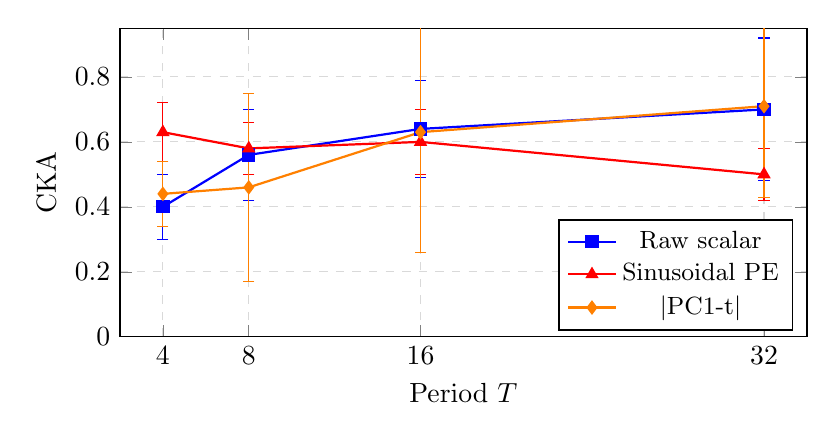
\begin{tikzpicture}
\begin{axis}[
    width=0.85\columnwidth,
    height=5.5cm,
    xlabel={Period $T$},
    ylabel={CKA},
    xmin=2, xmax=34,
    ymin=0, ymax=0.95,
    xtick={4,8,16,32},
    legend style={at={(0.98,0.02)}, anchor=south east, font=\small},
    grid=major,
    grid style={dashed, gray!30},
]
\addplot[color=blue, mark=square*, thick, error bars/.cd, y dir=both, y explicit]
coordinates {
    (4, 0.40) +- (0, 0.10)
    (8, 0.56) +- (0, 0.14)
    (16, 0.64) +- (0, 0.15)
    (32, 0.70) +- (0, 0.22)
};
\addlegendentry{Raw scalar}

\addplot[color=red, mark=triangle*, thick, error bars/.cd, y dir=both, y explicit]
coordinates {
    (4, 0.63) +- (0, 0.09)
    (8, 0.58) +- (0, 0.08)
    (16, 0.60) +- (0, 0.10)
    (32, 0.50) +- (0, 0.08)
};
\addlegendentry{Sinusoidal PE}

\addplot[color=orange, mark=diamond*, thick, error bars/.cd, y dir=both, y explicit]
coordinates {
    (4, 0.44) +- (0, 0.10)
    (8, 0.46) +- (0, 0.29)
    (16, 0.63) +- (0, 0.37)
    (32, 0.71) +- (0, 0.28)
};
\addlegendentry{$|$PC1-t$|$}
\end{axis}
\end{tikzpicture}
\caption{CKA with engineered encodings and |PC1-timestep correlation| as a function of period $T$ (mean $\pm$ std across 5 seeds). Similarity to raw scalar encoding increases at longer horizons, while similarity to sinusoidal PE decreases.}
\label{fig:scaling}
\end{figure}

\section{Discussion}

LSTM-based RL agents do not converge to a single canonical temporal code.
The code they learn depends on their initialization, and which engineered encoding it resembles shifts with the task's temporal horizon.
These findings have implications at several levels.

\textbf{Conceptual implication: no canonical internal clock.}
The assumption that recurrent networks provide a unified, well-defined temporal code is embedded in much of RL practice---for example, when comparing representations across seeds or architectures, or when interpreting hidden states as encoding specific task variables.
Our results indicate that, at least in simple periodic environments, this assumption does not hold: the framing of time is contingent on optimization path and task structure.
This has direct methodological implications: a study using only seed 42 would conclude ``LSTMs encode time via sinusoidal-like codes,'' while a study using only seed 456 would conclude ``LSTMs encode time via phase-based codes.''
Neither generalizes.

\textbf{Implications for interpretability.}
The representational plurality we observe raises a deeper question for RL interpretability: if the temporal code is not unique, what does it mean to ``interpret'' a neuron as a time cell?
The same functional role (phase discrimination) is implemented by different neuronal subpopulations across seeds.
This is consistent with \citet{edelman2001degeneracy}'s concept of degeneracy---structurally different elements performing the same function---and suggests that single-seed interpretability analyses may be misleading.

\textbf{Conceptual implications: what does ``representation'' mean in RL?}
If temporal codes are non-unique, then ``what the agent has learned'' is not a well-defined mapping from task to internal code, but one of many functionally equivalent solutions.
This is Edelman's \emph{degeneracy} (many-to-one structure-to-function mapping), not mere \emph{redundancy} (duplicate copies of the same structure): the solutions differ qualitatively, not just numerically.
If the representational code is path-dependent, then representation analysis characterizes one among many valid solutions, not a canonical internal structure.
Whether this plurality is a nuisance for interpretability or a genuine feature of learning systems remains an open question.

\textbf{Scope and limitations.}
We do not claim a universal taxonomy of temporal coding in RL.
Instead, we isolate a simple setting where temporal structure can be varied in a controlled way and representation geometry inspected directly.
Three caveats are worth flagging.
First, our experiments use one environment, one algorithm (REINFORCE), and one architecture (single-layer LSTM).
Second, at $T = 32$, training instability (2/5 seeds fail) limits the horizon analysis.
Third, CKA measures linear similarity and may miss nonlinear encoding strategies.
Future work should investigate whether representational plurality persists across architectures (GRUs, attention-based models) and in more complex domains.

\bibliographystyle{plainnat}
\bibliography{temporal_repr_refs}

\begin{appendices}

\section{Single-Neuron Phase Selectivity Analysis}
\label{app:neurons}

\begin{table}[h]
\centering
\caption{Top-8 time cell dimensions and preferred phases per seed (DoorGrid, $T = 4$).
Mean pairwise overlap: 1.8/8 dimensions (Jaccard $= 0.14$).
Hypergeometric expectation given 34/64 selective dims: $\approx 1.88$.}
\label{tab:tuning}
\begin{tabular}{ccc}
\toprule
\textbf{Seed} & \textbf{Top-8 dims} & \textbf{Preferred phases} \\
\midrule
42  & 28, 43, 7, 44, 31, 32, 50, 39 & 2, 2, 0, 1, 3, 1, 3, 2 \\
123 & 2, 40, 25, 49, 14, 4, 33, 36  & 1, 2, 3, 3, 3, 1, 3, 2 \\
456 & 40, 35, 44, 39, 36, 22, 26, 43 & 3, 2, 0, 0, 3, 2, 3, 2 \\
789 & 25, 51, 10, 15, 29, 18, 24, 38 & 1, 1, 1, 3, 3, 3, 3, 3 \\
1024 & 43, 10, 25, 11, 39, 4, 36, 40 & 3, 1, 2, 3, 2, 1, 3, 2 \\
\bottomrule
\end{tabular}
\end{table}

Hidden-unit indices are not aligned across independently trained models, so low overlap in unit indices is partially expected under permutation invariance.
With 34 of 64 dimensions showing high phase selectivity, the observed overlap (1.8/8) is close to the hypergeometric chance level ($\approx 1.88$), so this analysis does not provide evidence for or against representational uniqueness.
The population-level CKA differences provide the stronger signal: seed 42 has CKA(sin\_PE) $= 0.74$ while seed 456 has CKA(phase) $= 0.62$ with CKA(sin\_PE) $= 0.46$, indicating genuinely different encoding geometries.

\section{Failed Seeds at Long Horizons}
\label{app:failed}

At $T = 16$, seed 1024 fails to converge (best eval reward $= -2.0$).
At $T = 32$, seeds 456 and 789 fail to converge (best eval reward $= -2.0$).
The reported CKA statistics in Table~\ref{tab:scaling} include all 5 seeds, as even non-converged agents contain representational structure worth characterizing.
At $T = 32$, excluding the 2 failed seeds: CKA(raw) $= 0.61 \pm 0.28$ (vs.\ $0.70 \pm 0.22$ with all 5), and CKA(sin\_PE) $= 0.54 \pm 0.10$ (vs.\ $0.50 \pm 0.08$).
The same pattern holds---raw scalar still beats sin PE.

\end{appendices}

\end{document}
